\chapter{Prologue}
This summer, we will be making our way through Knapp's \emph{Lie Groups
  Beyond an Introduction} \cite{knapp} although, I (the writer of these
notes) will occasionally refer to \cite{hall} for examples.

Throughout these notes

\begin{tabular}{cl}
  $C_n$ &the cyclic group of order $n$\\
  $S_n$&the symmetric group on $n$ letters\\
  $A_n$&the alternating group on $n$ letters
\end{tabular}

\section{Representation of Finite Groups}
This section of the notes is mainly paraphrased from Fulton and Harris's
book \emph{Representation Theory}. We will quickly talk about the
representation theory of finite groups and move on to the representation
theory of Lie groups, covering perhaps the first 5 chapters of the latter
book.

\subsection{Definitions}
Throughout this section, by a \emph{representation} of a finite group $G$
we mean a homomorphism $\rho\colon G\to\GL(V)$, where $V$ is a
finite-dimensional complex vector space. A \emph{representation} of a
finite group $G$ on a finite-dimension; we say that such a map $\rho$
\emph{gives $V$ a $G$-module structure.} When there is little ambiguity
about the map $\rho$, we will call $V$ itself a representation of $G$; we
also suppress the symbol $\rho$ and write $g\bfv$ for $\rho(g)(\bfv)$
whenever context allows us. The dimension of $V$ is called the \emph{degree} of
$\rho$.

A map $\varphi$ between two representations $V$ and $W$ of $G$ is a vector
space map $\varphi\colon V\to W$ such that
\[
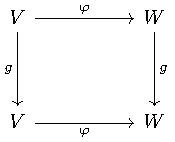
\includegraphics{figures/week-1-diag-1}
\]
commutes for every $g\in G$. We will call such a map a \emph{$G$-linear
  map} when we want to distinguish it from an arbitrary linear map between
the vector spaces $V$ and $W$. We can thus, then define $\Ker\varphi$,
$\Img\varphi$, and $\Coker\varphi$, which naturally inherit a $G$-module
structure from $V$.

A \emph{subrperesentation} of a representation $V$ is a vector subspace $W$
of $V$ which is invariant under the action by $G$, that is,
$g\bfw=\bfw$ for all $\bfw\in W$. A representation $V$ is called
\emph{irreducible} if there is no proper nonzero invariant subspace $W$ of
$V$.


As it turns out, some of if $V$ and $W$ are representations, so are
$V\oplus W$ and $V\otimes W$ with $g(v\otimes w)\coloneqq gv\otimes gw$,
and so are the $n$th tensor power $\bigotimes^nV$, the exterior power
$\bigwedge^n V$ and the symmetric powers $\Sym^n V$. The dual
$V^*=\Hom(V,\bbC)$ of $V$ is also a representation, though not in the most
obvious way: We want the two representations of $G$ with respect to the
natural pairing between $V$ and $V^*$, that is,
$\langle\bfv^*,\bfv\rangle\coloneqq\bfv^*(\bfv)$, so that if
$\rho\colon G\to\GL(V)$ is a representation and $\rho^*\colon G\to\GL(V)$
is its dual, then we have
\[
  \langle \rho^*(g)(\bfv^*),\rho(g)(\bfv) \rangle=\langle \bfv^*,\bfv \rangle
\]
for all $g\in G$, $\bfv\in V$, and $\bfv^*\in V^*$. This in turn forces us
to define the dual representation $\rho^*\colon V^*\to V^*$ by
\[
  \rho^*(g)\coloneqq\prescript{\rmt}{}{\rho}(g^{-1})
\]
for all $g\in G$. Let us verify that $\rho^*$ in fact satisfies $\langle
\rho^*(g)(\bfv^*),\rho(g)(\bfv) \rangle=\langle\bfv^*,\bfv \rangle$: Let
$\bfv^*\in V^*$ and $\bfv\in V$,
then
\begin{align*}
  \langle\rho^*(g)(\bfv^*),\rho(g)(\bfv)\rangle
  &=\langle\prescript{t}{}\rho(g^{-1})(\bfv^*),\rho(g)(\bfv)\rangle\\
  &=\langle \bfv^*,\rho(g^{-1})\circ\rho(g)(\bfv)\rangle\\
  &=\langle \bfv^*,\bfv\rangle.
\end{align*}

Having defined the dual representation of the tensor product of two
representations, it is likewise the case that if $V$ and $W$ are
representations, then $\Hom(V,W)$ is also a representation, via the
identification $\Hom(V,W)=V^*\otimes W$. Unraveling this, if we view an
element of $\Hom(V,W)$ as a linear map $\varphi$ from $V$ to $W$, we have
\[
(g\varphi)(v)=g\varphi(g^{-1}v)
\]
for all $v\in V$. In other words, the definition is such that the diagram
\[
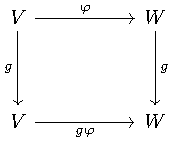
\includegraphics{figures/week-1-diag-2}
\]
commutes. Note that the dual representation is, in turn, a special case of
this: When $W=\bbC$ is the trivial representation, i.e., $gw=w$ for all
$w\in\bbC$, this makes $V^*$ into a $G$-module, with
$g\varphi(v)=\varphi(g^{-1}v)$, i.e.,
$g\varphi=\prescript{\rmt}{}{(g^{-1})}$.

\begin{exercise}
We verify that in general the vector space of $G$-linear maps between two
representations $V$ and $W$ of $G$ is just the subspace $\Hom(V,W)^G$ of
elements of $\Hom(V,G)$ fixed under the action of $G$. We will often denote
this space by $\Hom_G(V,W)$.
\end{exercise}
\begin{proof}
\end{proof}

We have taken the identification $\Hom(V,W)=V^*\otimes W$ as the
definition of the representation $\Hom(V,W)$. More generally, the usual
identities for vector spaces are also true for representations, e.g.,
\begin{align*}
V\otimes(U\oplus W)&=(V\otimes U)\oplus(V\otimes W)\\
\bigwedge^k(V\oplus W)&=\bigoplus_{a+b=k}{\textstyle\bigwedge^a V\otimes\bigwedge^b
  W}\\
{\textstyle\bigwedge^k V^*}&=\left({\textstyle{\bigwedge^kV}}\right)^*
\end{align*}

If $X$ is any finite set and $G$ acts on the left on $X$, i.e.,
$G\to\Aut(X)$ is a homomorphism to the premutation group of $X$, there is
an associated permutation representation: Let $V$ be the vector space with
basis $\{\bfe_x:x\in X\}$, and let $G$ act on $V$ by
\[
  g\cdot\sum a_x\bfe_x\coloneqq\sum a_x\bfe_{gx}.
\]
The regular representation, denoted $R_G$ or simply $R$, corresponds to the
left action of $G$ on itself. Alternatively, $R$ is the space of
complex-valued functions on $G$, where an element $g\in G$ acts on a
function $\alpha$ by $(g\alpha)(h)=\alpha(g^{-1}h)$.

\subsection{Complete Reducibility; Schur's Lemma}
Before we begin classifying the representations of a finite group $G$ we
should try to simplify life by restricting our search
somewhat. Specifically, we have seen that representations of $G$ can be
built up out of other representations by linear algebraic operations, most
simply by taking the direct sum. We should focus, then, on representations
that are ``atomic'' with respect to this operation, i.e., that cannot be
expressed as a direct sum of others; the usual term for such a
representation is \emph{indecomposable}. Happily, this situation is as nice
as it could possibly be: A representation is atomic in this sense if and
only if it is irreducible (i.e., contains no proper subrepresentations);
and every representation is the direct sum of irreducibles, in a suitable
sense uniquely so. The key to all this is
\begin{proposition}
If $W$ is a subrepresentation of a representation $V$ of a finite group
$G$, then there is an elementary invariant subspace $W'$ of $V$, so that
$V=W\oplus W'$.
\end{proposition}
\begin{proof}
  There are two ways of showing this. One can introduce a positive definite
  Hermitian inner product $H$ on $V$ which is preserved by each $g\in G$
  (i.e., such that $H(g\bfv,g\bfw)=H(\bfv,\bfw)$ for all $\bfv,\bfw\in V$,
  $g\in G$). Indeed, if $H_0$ is any Hermitian product on $V$, one gets
  such an $H$ by averaging over $G$:
  \begin{equation}
    \label{eq:1:hermitian-inn-prod}
    H(\bfv,\bfw)\coloneqq\sum_{g\in G}H_0(g\bfv,g\bfw).
  \end{equation}
  Then the perpendicular subspace $W^\perp$ is complementary to $W$ in
  $V$. Alternatively, we can simply choose an arbitrary subspace $U$
  complementary to $W$, let $\pi_0\colon V\to W$ be the projection given by
  the direct sum decomposition $V=W\oplus U$, and average the map $\pi_0$
  over $G$: i.e., take
  \begin{equation}
    \label{eq:1:averaging-map}
    \pi(\bfv)\coloneqq\sum_{g\in G}g(\pi_0(g^{-1}\bfv)).
  \end{equation}
  this will then be a $G$-linear map from $V$ onto $W$, which is
  multiplication by $|G|$ on $W$; its kernel will, therefore, be a subspace
  of $V$ invariant under $G$ and complemnetary to $W$.
\end{proof}

\begin{corollary}
  Any representation is a direct sum of irreducible representations.
\end{corollary}

This property is called complete reducibility, or semisimplicity. We will
see that, for continuous representations, the circle $S^1$, or any compact
group, has this property; integration over the group (with respect to an
invariant measure on the group) plays the role of averaging in the above
proof. The (additive) group $\bbR$ does not have this property: The
representation
\[
  a\longmapsto
  \begin{bmatrix}
    1&a\\0&1
  \end{bmatrix}
\]
leaves the $x$ axis fixed, but there is no complementary subspace. We will
see other Lie groups such as $\SL_n(\bbC)$ that are semisimple in this
sense. Note also that this argument would fail if the vector space $V$ was
over a field of finite characteristic since it might then be the case that
$\pi(\bfv)=\mathbf{0}$ for for $\bfv\in W$. The failure, of complete
reducibility is one  of is one of the things that makes the subject of
modular representations, or representations on vector spaces over finite
fields, so tricky.

The extent to which the decomposition of an arbitrary representation into a
direct sum of irreducible ones is unique is one of the consequences of the
following:

\begin{theorem}[Schur's lemma]
  If $V$ and $W$ are irreducible representations of $G$ and $\varphi\colon
  V\to W$ is a $G$-module homomorphism, the
  \begin{enumerate}[label=\textnormal{(\alph*)},noitemsep]
  \item Either $\varphi$ is an isomorphism, or $\varphi=\mathbf{0}$.
  \item If $V=W$, then $\varphi=\lambda\cdot I$ for some $\lambda\in\bbC$,
    $I$ being the identity.
  \end{enumerate}
\end{theorem}
\begin{proof}
  The first claim follows from the fact that $\Ker\varphi$ and
  $\Img\varphi$ are invariant subspaces. For the second, since $\bbC$ is
  algebraically closed, $\varphi$ must have an eigenvalue $\lambda$, i.e.,
  for some $\lambda\in\bbC$, $\varphi-\lambda I$ has a nonzero kernel. By
  Theorem 1, we must have $\varphi-\lambda I=\mathbf{0}$ so $\varphi=\lambda I$.
\end{proof}

We can summarize what we have shown thus far in
\begin{proposition}
  For any representation $V$ of a finite group $G$, there is a
  decomposition
  \[
    V=V_1^{\oplus a_1}\oplus\dotsb\oplus V_k^{\oplus a_k},
  \]
  where the $V_i$ are distinct irreducible representations. The
  decomposition of $V$ into a direct sum of the $k$ factors is unique, as
  are the $V_i$ that occur and their multiplicities $a_i$.
\end{proposition}
\begin{proof}
It follows from Schur's lemma that if $W$ is another representation of $G$,
with decomposition $W=\bigoplus W_j^{\oplus b_j}$, and $\varphi\colon V\to
W$ is a map of representations, then $\varphi$ must map the factor
$V_i^{\oplus a_i}$ into that factor $W_j^{\oplus b_j}$ for which $W_j\simeq
V_i$; when applied to the identity map of $V$ to $V$, the stated uniqueness
follows.
\end{proof}


Occasionally, the decomposition is written
\[
V=a_1V_1\oplus\dotsb\oplus a_kV_k=a_1V_1+\dotsb+a_kV_k,
\]
especially when one is encountered only about the isomorphism classes and
multiplicities of the $V_i$.

One more fact that will be established in the following lecture is that a
finite group $G$ admits only finitely many irreducible representations
$V_i$ up to isomorphism (in fact, we can say how many).

Our first goal, in analyzing the representations of any group, will
therefore be:
\begin{enumerate}[label=(\alph*)]
\item Described all the irreducible representations of $G$.

  Once we have done this, there remains the problem of carrying out in
  practice the description of a given representation in these terms. Thus,
  our second goal will be:
\item Find techniques for giving the direct sum decomposition, and in
  particular determining the multiplicities $a_i$ of an arbitrary
  representation $V$.

  Finally, it is the case that the representations we will most often be
  concerned with are those arising from simpler ones by the sort of linear-
  or miltilinear-algebraic operations described above. We would like,
  therefore, to be able to describe, in the terms above, the representation
  we get when we perform these operations on a know representation. This is
  known generally as
\item Plethysm: Describe the decompositions, with multiplicities, of
  representations derived from a given representation $V$, such as
  $V\otimes V$, $V^*$, $\bigwedge^k V$, $\Sym^k V$ and
  $\bigwedge^k(\bigwedge^\ell V)$. Note that if $V$ decomposes into a sum
  of two representations, these representatinos decompose accordingly;
  e.g., if $V=U\oplus W$, then
  \[
    \bigwedge^k V=\bigoplus_{i+j=k}\bigwedge^i U\otimes\bigwedge^j W,
  \]
  so it is enough to work out this plethysm for irreducible
  representations. Similarly, if $V$ and $W$ are two irreducible
  representations, we want to decompose $V\otimes W$; this is usually known
  as the Clebsch--Gordan problem.
\end{enumerate}
\subsection{Examples: Abelian Groups; $S_3$}
One obvious place to look for examples is with Abelian groups. It does not
take long, however, to deal with this case. Basically, we may obverve in
general that if $V$ is a representation of the finite group $G$, abelian or
not, each $g\in G$ gives a map $\rho(g)\colon V\to V$; but this map is not
generally a $G$-module homomorphism: For general $h\in G$, we will have
\[
g(h(\bfv))\neq h(g(\bfv)).
\]
Indeed, $\rho(g)\colon V\to V$ will be $G$-linear for every $\rho$ if and
only if $g$ is in the center $Z(G)$ of $G$. In particular, if $G$ is
Abelian, and $V$ is an irreducible representation, then by Schur's lemma
every element $g\in G$ acts on $V$ by a scalar multiple of the
identity. Every subspace of $V$ is thus invariant; so that $V$ must be one
dimensional. The irreducible representations of an Abelian group $G$ are
thus simply elements of the dual group, i.e., homomorphism $\rho\colon
G\to\bbC^*$.

We begin with the next simplest nonAbelian group, $G\coloneqq S_3$. To
begin with, we have two one-dimensional representations: We have the
trivial representation, which we shall denote $U$, and the alternating
representation $U'$, defined by setting
\[
gv=\sgn(g)v
\]
for $g\in G$, $v\in\bbC$. Next, since $G$ comes to us as a permutation
group, we have a natural permutation representation, in which $G$ acts on
$\bbC^3$ by permuting the coordinates. Explicitly, if
$\{\bfe_1,\bfe_2,\bfe_3\}$ is the standard basis, then
$g\cdot\bfe_i=\bfe_{g(i)}$, or equivalently,
\[
g\cdot (z_1,z_2,z_3)=\left(z_{g^{-1}(1)},z_{g^{-1}(2)},z_{g^{-1}(3)}\right).
\]
This representation, like any permutation representation, is not
irreducible: The line spanned by the sum $(1,1,1)$ of the basis vectors is
invariant, with complementary subspace
\[
V\coloneqq\left\{\,(z_1,z_2,z_3)\in\bbC^3:z_1+z_2+z_3=0\,\right\}.
\]
This two-dimensional representation of $V$ is easily seen to be
irreducible; we call it the standard representation of $S_3$.

Let us now turn to the problem of describing an arbitrary representation of
$S_3$. We will see in the next lecture that a wonderful tool for doing this
is called \emph{character theory}; but, as inefficient as this may be, we
would like here to adapt the more ad hoc approach.

We have just seen that the representation theory of a finite Abelian group
is virtually trivial, we will start our analysis of an arbirtary
representation $W$ of $S_3$ by looking just at the action of the Abelian
subgroup $A_3=C_3\subset S_3$. This yields a very simple decomposition: If
we take $\tau$ to be any generator of $A_3$ (that is, any $3$-cycle), the
space $W$ is spanned by eigenvectors $\bfv_i$ for the action $\tau$, whose
eigenvalues are of course all powers of the cube root of unity
$\omega\coloneqq e^{2\pi i/3}$. Thus,
\[
W=\bigoplus V_i,
\]
where
\[
V_i\coloneqq\bbC\bfv_i
\]
and
\[
\tau\bfv_i=\omega^{\alpha_i}\bfv_i.
\]

Next, we ask how the remaining elements of $S_3$ act on $W$ in terms of
this decomposition. TO see how it goes, let $\sigma$ be any transposition,
so that $\tau$ and $\sigma$, together generate $S_3$, with the relation
$\sigma\tau\sigma=\tau^2$. We want to know where $\sigma$ sends an
eigenvector $\bfv$ for the action of $\tau$, say with eigenvalue
$\omega^i$; to answer this, we look at how $\tau$ acts on
$\sigma(\bfv)$. We use the basic relation above to write
\[
  \begin{aligned}
    \tau(\sigma(\bfv))
    &=\sigma(\tau^2(\bfv))\\
    &=\sigma(\omega^{2i}\bfv)\\
    &=\sigma^{2i}\sigma(bfv).
  \end{aligned}
\]
The conclusion, then, is that if $\bfv$ is an eigenvector for $\tau$ with
eigenvalue $\omega^i$, then $\sigma(\bfv)$ is again an eigenvector for
$\tau$, with eigenvalue $\omega^{2i}$.


\section{Characters}
\subsection{Characters}
As it turns out, there is a remarkably effective tool for understanding the
representations of a finite group $G$, called \emph{character theory}. This
is in some ways motivated by the example worked out in the last section
where we saw that a representation of $S_3$ was determined by knowing the
eigenvalues of the action of the elements $\tau$ and $\sigma\in S_3$. For a
general group $G$, it is not clear what subgroups and or elements should
play the role of $A_3$, $\tau$, and $\sigma$; but the example certainly
suggests that knowing all the eigenvalues of each element of $G$ should
suffice to describe the representation.

Of course, specifying all the eigenvalues of the action of each element of
$G$ is somewhat unwieldy; but fortunately, it is redundant as well. For
example, if we know that the eigenvalues $\{\lambda_i\}$ of an element
$g\in G$, then of course we know the eigenvalues $\{\lambda_i^k\}$ of $g^k$
for each $k$ as well. We can thus use this redundancy to simplify the data
we have to specify.

\begin{definition}
If $V$ is a representation of $G$, its \emph{character $\chi_V$} is the
complex-valued function on the group defined by
\[
\chi_V\coloneqq\tr\bigr(g|_V\bigl).
\]
the trace of $g$ on $V$.
\end{definition}

In particular, we have
\[
\chi_V(hgh^{-1})=\chi_V(g)
\]
so that $\chi_V$ is constant on the conjugacy classes of $G$; such a
function is called a \emph{class function}. Note that $\chi_V(1)=\dim V$.

\begin{proposition}
Let $V$ and $W$ be representations of $G$. Then
\[
  \begin{aligned}
    \chi_{V\oplus W}&=\chi_V+\chi_W,&\chi_{V\otimes W}&=\chi_V\chi_W\\
    \chi_{V^*}&=\bar\chi_V&\chi_{\wedge^2
      V}(g)&=\tfrac{1}{2}\left[\chi_V(g)^2-\chi_V(g^2)\right].
  \end{aligned}
\]
\end{proposition}
\begin{proof}
\end{proof}



%%% Local Variables:
%%% mode: latex
%%% TeX-master: "../MA598-Lie-Groups"
%%% End:
